\documentclass[aspectratio=169,10pt]{beamer}

\usepackage{array}
\usepackage{booktabs}
\usepackage{graphicx}
\usepackage{amsmath}
\usepackage{amssymb}
\usepackage{tikz}
\usetikzlibrary{arrows.meta,calc,positioning,shapes.geometric,fit}
\newcolumntype{L}[1]{>{\raggedright\arraybackslash}p{#1}}

% DGIST ISL Custom Color Palette
\definecolor{islteal}{RGB}{43,133,147}
\definecolor{islred}{RGB}{203,76,65}
\definecolor{isldark}{RGB}{52,61,67}
\definecolor{islnavy}{RGB}{31,55,95}
\definecolor{islmuted}{RGB}{92,101,108}
\definecolor{isllight}{RGB}{236,241,243}
\definecolor{islgold}{RGB}{184,119,20}
\definecolor{islgreen}{RGB}{44,145,91}
\definecolor{islpurple}{RGB}{130,58,160}

\newcommand{\deckdate}{2026.08.21}
\newcommand{\labname}{DGIST Intelligent Systems and Learning Laboratory}

\setbeamersize{text margin left=0.65cm,text margin right=0.65cm}
\setbeamertemplate{navigation symbols}{}
\setbeamertemplate{blocks}[rounded][shadow=false]
\setbeamercolor{normal text}{fg=isldark,bg=white}
\setbeamercolor{frametitle}{fg=isldark,bg=white}
\setbeamercolor{footer}{fg=white,bg=isldark}
\setbeamerfont{frametitle}{series=\bfseries,size=\Large}
\setbeamerfont{normal text}{size=\small}

\setbeamertemplate{frametitle}{%
  \nointerlineskip%
  \begin{beamercolorbox}[wd=\paperwidth,ht=1.35cm,dp=0cm]{frametitle}
    \vskip0.45cm%
    \hspace*{0.74cm}\insertframetitle\par%
    \vskip0.05cm%
    \hspace*{0.74cm}{\color{islteal}\rule{0.68\paperwidth}{4pt}}%
    {\color{islred}\rule{0.20\paperwidth}{4pt}}%
  \end{beamercolorbox}%
}

\setbeamertemplate{footline}{%
  \leavevmode%
  \begin{beamercolorbox}[wd=\paperwidth,ht=0.34cm,dp=0.11cm]{footer}
    \hspace*{0.65cm}{\scriptsize\deckdate}%
    \hfill{\scriptsize Reinforcement Learning \& Robotics Track \quad $\vert$ \quad Week 04: Replay \& Target Networks}\hfill%
    {\scriptsize\insertframenumber\,/\,\inserttotalframenumber}\hspace*{0.65cm}%
  \end{beamercolorbox}%
}

\newcommand{\bottomrulebar}{%
  \begin{tikzpicture}[remember picture,overlay]
    \fill[islteal] (current page.south west) rectangle ++(0.43\paperwidth,0.11cm);
    \fill[isldark] ([xshift=0.43\paperwidth]current page.south west)
      rectangle ++(0.34\paperwidth,0.11cm);
    \fill[islred] ([xshift=0.77\paperwidth]current page.south west)
      rectangle ++(0.23\paperwidth,0.11cm);
  \end{tikzpicture}%
}

\newcommand{\sectionlabel}[1]{%
  {\small\bfseries\color{islteal}#1}\par\vspace{0.14cm}%
}

\begin{document}

% ==========================================
% SLIDE 1: Title Slide
% ==========================================
\begin{frame}[plain,noframenumbering]
  \bottomrulebar
  \vspace{1.00cm}
  {\centering
    {\fontsize{22}{26}\selectfont\bfseries\color{islnavy}
      Week 04: Replay Buffers \& Target Networks\par}
    \vspace{0.22cm}
    {\fontsize{15}{18}\selectfont\color{islteal}
      What Replay and Delayed Targets Change---and What They Do Not Prove\par}
    \vspace{0.50cm}
    {\large\bfseries Reinforcement Learning \& Robot Learning Core Curriculum\par}
    \vspace{0.20cm}
    {\small Presented by \textbf{DGIST ISL Team}\par}
    \vspace{0.12cm}
    {\small\color{islmuted} \labname\par}
    \vspace{0.10cm}
    {\small \deckdate\par}
    \vspace{0.45cm}
    {\scriptsize\color{islmuted}
      Core Concepts: Deadly Triad $\cdot$ Temporal Decorrelation $\cdot$ Moving Targets $\cdot$ Multi-Seed Ablation\par}
  }
\end{frame}

% ==========================================
% SLIDE 2: The Deadly Triad & Instability
% ==========================================
\begin{frame}{The Deadly Triad: Why Instability Can Appear}
  \sectionlabel{Function approximation, bootstrapping, and off-policy learning can interact poorly}

  {\centering
    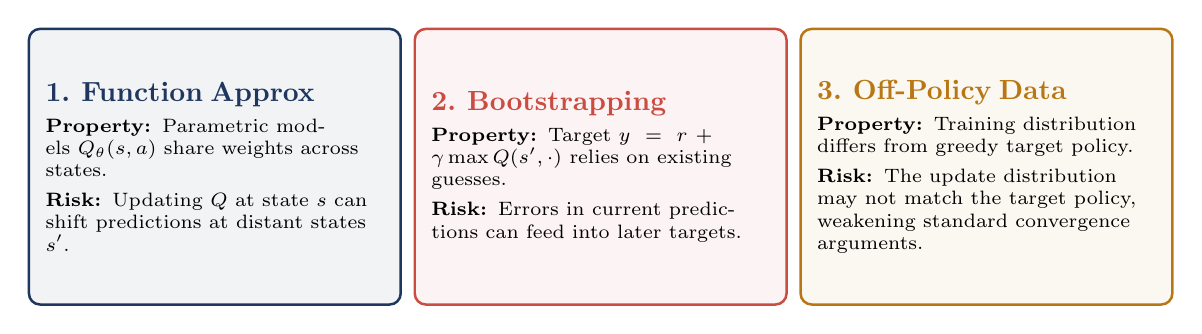
\begin{tikzpicture}[
      pillar/.style={rounded corners=4pt, text width=4.3cm, minimum height=3.5cm, align=left, inner sep=6pt, font=\scriptsize, line width=0.9pt}
    ]
      % Pillar 1: Function Approx
      \node[pillar, draw=islnavy, fill=islnavy!6] (p1) at (2.4, 1.9) {
        {\normalsize\bfseries\color{islnavy} 1. Function Approx}\\[3pt]
        \textbf{Property:} Parametric models $Q_\theta(s, a)$ share weights across states.\\[3pt]
        \textbf{Risk:} Updating $Q$ at state $s$ can shift predictions at distant states $s'$.
      };

      % Pillar 2: Bootstrapping
      \node[pillar, draw=islred, fill=islred!6] (p2) at (7.3, 1.9) {
        {\normalsize\bfseries\color{islred} 2. Bootstrapping}\\[3pt]
        \textbf{Property:} Target $y = r + \gamma \max Q(s', \cdot)$ relies on existing guesses.\\[3pt]
        \textbf{Risk:} Errors in current predictions can feed into later targets.
      };

      % Pillar 3: Off-Policy
      \node[pillar, draw=islgold, fill=islgold!6] (p3) at (12.2, 1.9) {
        {\normalsize\bfseries\color{islgold} 3. Off-Policy Data}\\[3pt]
        \textbf{Property:} Training distribution differs from greedy target policy.\\[3pt]
        \textbf{Risk:} The update distribution may not match the target policy, weakening standard convergence arguments.
      };
    \end{tikzpicture}
  \par}
\end{frame}

% ==========================================
% SLIDE 3: Stabilizer 1 - Experience Replay
% ==========================================
\begin{frame}{Stabilizer 1: Circular Experience Replay Buffer}
  \sectionlabel{Spreading sample sets across stored time without claiming literally i.i.d. data}

  {\centering
    \begin{tikzpicture}[
      box/.style={rounded corners=4pt, text width=6.5cm, minimum height=3.2cm, inner sep=6pt, font=\scriptsize, line width=0.9pt, align=left}
    ]
      % Left: Sequential Correlation
      \node[box, draw=islred, fill=islred!6] at (3.5, 1.7) {
        {\bfseries\color{islred}\normalsize Sequential Window ($B=32$)}\\[3pt]
        $\bullet$ Transitions arrive sequentially: $(s_t, a_t, r_t, s_{t+1})$.\\[2pt]
        $\bullet$ \textbf{Mean all-pairs index gap:} $11.00$.\\[2pt]
        $\bullet$ \textbf{Adjacent all-pair rate:} $6.2\%$.\\[2pt]
        $\bullet$ The window covers one contiguous timeline segment.
        \vskip4pt
        \centering
        \begin{tikzpicture}[scale=0.7]
          \draw[thick, fill=islred!20] (0,0) circle (0.3) node{\tiny $s_0$};
          \draw[-{Latex}, thick] (0.3,0) -- (1.0,0);
          \draw[thick, fill=islred!20] (1.3,0) circle (0.3) node{\tiny $s_1$};
          \draw[-{Latex}, thick] (1.6,0) -- (2.3,0);
          \draw[thick, fill=islred!20] (2.6,0) circle (0.3) node{\tiny $s_2$};
        \end{tikzpicture}
      };

      % Right: Replay Decoupling
      \node[box, draw=islteal, fill=islteal!6] at (10.7, 1.7) {
        {\bfseries\color{islteal}\normalsize Uniform Replay Sampling}\\[3pt]
        $\bullet$ Store $N$ past transitions in FIFO buffer $\mathcal{D}$.\\[2pt]
        $\bullet$ Draw uniform minibatches: $\{e_i \sim \mathcal{D}\}_{i=1}^B$.\\[2pt]
        $\bullet$ \textbf{Mean all-pairs index gap:} $76.92$.\\[2pt]
        $\bullet$ \textbf{Adjacent all-pair rate:} $0.6\%$.\\[2pt]
        $\bullet$ Spans stored time broadly; does not prove i.i.d.
        \vskip4pt
        \centering
        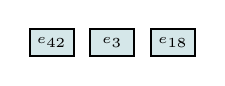
\begin{tikzpicture}[scale=0.7]
          \draw[thick, fill=islteal!20] (0,0) rectangle (0.8,0.5) node[pos=.5]{\tiny $e_{42}$};
          \draw[thick, fill=islteal!20] (1.1,0) rectangle (1.9,0.5) node[pos=.5]{\tiny $e_{3}$};
          \draw[thick, fill=islteal!20] (2.2,0) rectangle (3.0,0.5) node[pos=.5]{\tiny $e_{18}$};
        \end{tikzpicture}
      };
    \end{tikzpicture}
  \par}
\end{frame}

% ==========================================
% SLIDE 4: Stabilizer 2 - Target Network
% ==========================================
\begin{frame}{Stabilizer 2: Frozen Target Networks}
  \sectionlabel{Slowing one source of target motion with piecewise-frozen parameters}

  {\centering
    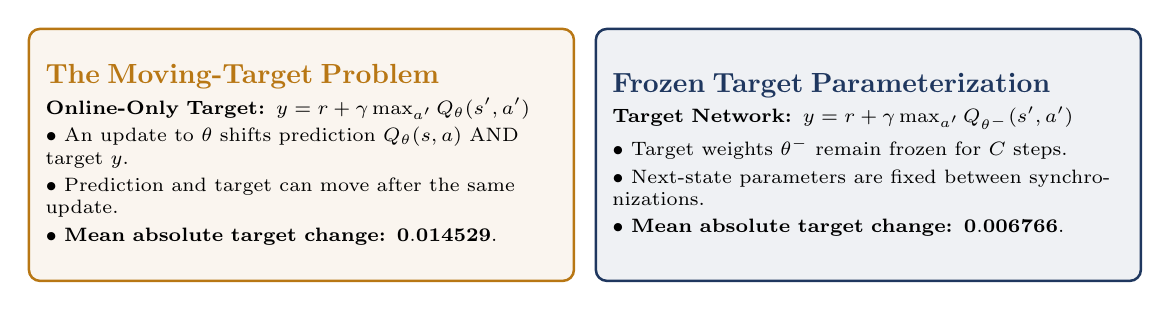
\begin{tikzpicture}[
      card/.style={rounded corners=4pt, text width=6.5cm, minimum height=3.2cm, align=left, inner sep=6pt, font=\scriptsize, line width=0.9pt}
    ]
      % Left: Online moving target
      \node[card, draw=islgold, fill=islgold!7] at (3.5, 1.7) {
        {\bfseries\color{islgold}\normalsize The Moving-Target Problem}\\[3pt]
        \textbf{Online-Only Target:} $y = r + \gamma \max_{a'} Q_\theta(s', a')$\\[2pt]
        $\bullet$ An update to $\theta$ shifts prediction $Q_\theta(s, a)$ AND target $y$.\\[2pt]
        $\bullet$ Prediction and target can move after the same update.\\[2pt]
        $\bullet$ \textbf{Mean absolute target change:} $\mathbf{0.014529}$.
      };

      % Right: Frozen target net
      \node[card, draw=islnavy, fill=islnavy!7] at (10.7, 1.7) {
        {\bfseries\color{islnavy}\normalsize Frozen Target Parameterization}\\[3pt]
        \textbf{Target Network:} $y = r + \gamma \max_{a'} Q_{\theta^-}(s', a')$\\[2pt]
        $\bullet$ Target weights $\theta^-$ remain frozen for $C$ steps.\\[2pt]
        $\bullet$ Next-state parameters are fixed between synchronizations.\\[2pt]
        $\bullet$ \textbf{Mean absolute target change:} $\mathbf{0.006766}$.
      };
    \end{tikzpicture}
  \par}
\end{frame}

% ==========================================
% SLIDE 5: Full DQN Training Loop
% ==========================================
\begin{frame}{System Architecture: The Stabilized DQN Loop}
  \sectionlabel{Interaction flow between environment, buffer, online network, and target network}

  {\centering
    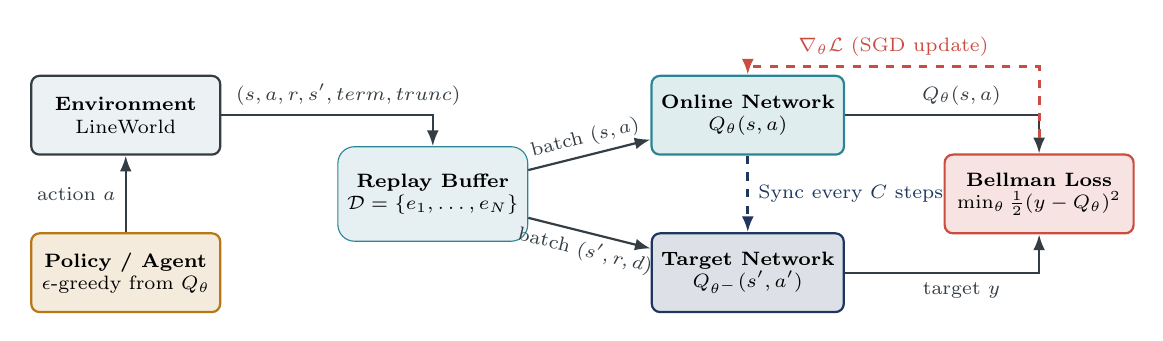
\begin{tikzpicture}[
      box/.style={rectangle, rounded corners=3pt, minimum width=2.4cm, minimum height=1.0cm, align=center, draw=isldark, line width=0.8pt, font=\scriptsize},
      data/.style={rectangle, rounded corners=6pt, draw=islteal, fill=islteal!12, minimum width=2.2cm, minimum height=1.2cm, font=\scriptsize, align=center},
      arr/.style={-{Latex[length=2.0mm]}, thick, color=isldark}
    ]
      % Left: Env and Agent
      \node[box, fill=isllight] (env) at (1.5, 3.1) {\textbf{Environment}\\LineWorld};
      \node[box, fill=islgold!15, draw=islgold] (policy) at (1.5, 1.1) {\textbf{Policy / Agent}\\$\epsilon$-greedy from $Q_\theta$};

      % Center: Replay Buffer
      \node[data] (buffer) at (5.4, 2.1) {\textbf{Replay Buffer}\\$\mathcal{D} = \{e_1, \dots, e_N\}$};

      % Right: Networks
      \node[box, fill=islteal!15, draw=islteal] (q_online) at (9.4, 3.1) {\textbf{Online Network}\\$Q_\theta(s, a)$};
      \node[box, fill=islnavy!15, draw=islnavy] (q_target) at (9.4, 1.1) {\textbf{Target Network}\\$Q_{\theta^-}(s', a')$};

      % Far Right: Loss Node
      \node[box, fill=islred!15, draw=islred] (loss) at (13.1, 2.1) {\textbf{Bellman Loss}\\$\min_\theta \tfrac{1}{2}(y - Q_\theta)^2$};

      % Paths
      \draw[arr] (policy) -- (env) node[midway, left]{\scriptsize action $a$};
      \draw[arr] (env) -| (buffer.north) node[pos=0.3, above]{\scriptsize $(s,a,r,s',term,trunc)$};
      \draw[arr] (buffer) -- (q_online) node[midway, above=-1pt, sloped]{\scriptsize batch $(s, a)$};
      \draw[arr] (buffer) -- (q_target) node[midway, below=-1pt, sloped]{\scriptsize batch $(s', r, d)$};
      \draw[arr] (q_online) -| (loss.north) node[pos=0.3, above]{\scriptsize $Q_\theta(s,a)$};
      \draw[arr] (q_target) -| (loss.south) node[pos=0.3, below]{\scriptsize target $y$};

      \draw[arr, dashed, color=islred, line width=1pt] (loss.north) ++(0, 0.2) -- ++(0, 0.9) -| (q_online.north) node[pos=0.25, above]{\scriptsize $\nabla_\theta \mathcal{L}$ (SGD update)};
      \draw[arr, dashed, color=islnavy, line width=1pt] (q_online.south) -- (q_target.north) node[midway, right]{\scriptsize Sync every $C$ steps};
    \end{tikzpicture}
  \par}
\end{frame}

% ==========================================
% SLIDE 6: Multi-Seed Four-Way Ablation Study
% ==========================================
\begin{frame}{Empirical Evidence: A Valid Null Result}
  \sectionlabel{Four linear-Q variants, 5 seeds, equal interaction/update budgets, fixed evaluation starts}

  \renewcommand{\arraystretch}{1.20}
  \setlength{\tabcolsep}{6pt}
  {\centering
    \footnotesize
    \begin{tabular}{@{}lcccc@{}}
      \toprule
      \textbf{Ablation Variant} & \textbf{Mean Return} & \textbf{Seed Std} & \textbf{Updates} & \textbf{Success Rate} \\
      \midrule
      \textbf{Online Only} & $0.9850$ & $0.0000$ & $393$ & $100\%$ \\
      \textbf{Target Only} & $0.9850$ & $0.0000$ & $393$ & $100\%$ \\
      \textbf{Replay Only} & $0.9850$ & $0.0000$ & $393$ & $100\%$ \\
      \textbf{Replay + Target} & $0.9850$ & $0.0000$ & $393$ & $100\%$ \\
      \bottomrule
    \end{tabular}
  \par}

  \vspace{0.10cm}
  {\centering\scriptsize All rows: 400 interactions and 393 optimizer steps. Replay rows use $B=8$; non-replay rows use $B=1$, so compute is not matched.\par}

  \vspace{0.16cm}
  \begin{columns}[T,onlytextwidth]
    \column{0.48\textwidth}
      \begin{block}{\small\color{islgold}\textbf{Supported Claim}}
        \footnotesize Under this exact LineWorld protocol, every configuration learned the same right-moving policy.
      \end{block}
    \column{0.48\textwidth}
      \begin{block}{\small\color{islgreen}\textbf{Unsupported Claim}}
        \footnotesize The experiment does not rank the stabilizers. LineWorld is too easy to reveal a policy-level advantage.
      \end{block}
  \end{columns}
\end{frame}

% ==========================================
% SLIDE 7: Hard vs Soft Target Updates
% ==========================================
\begin{frame}{Target Synchronization: Hard vs Soft Updates}
  \sectionlabel{Two standard paradigms for slowing target-parameter motion}

  \begin{columns}[T,onlytextwidth]
    \column{0.48\textwidth}
      {\small\bfseries\color{islteal} Periodic Hard Updates ($C$ steps)}\par\vspace{0.08cm}
      {\footnotesize
      $\bullet$ Copy weights abruptly every $C$ optimizer steps:
      $$\theta^- \leftarrow \theta \quad \text{every } C \text{ updates}$$
      $\bullet$ \textbf{Advantage:} Target parameters are fixed between copies.\\[2pt]
      $\bullet$ \textbf{Tradeoff:} Targets can jump at synchronization.}

    \column{0.48\textwidth}
      {\small\bfseries\color{islnavy} Continuous Soft Updates ($\tau$-Averaging)}\par\vspace{0.08cm}
      {\footnotesize
      $\bullet$ Interpolate weights continuously on every step:
      $$\theta^- \leftarrow \tau \theta + (1 - \tau)\theta^- \quad (\tau \approx 0.005)$$
      $\bullet$ \textbf{Advantage:} Usually smoother target-parameter motion.\\[2pt]
      $\bullet$ Standard in continuous Actor-Critic methods (DDPG, SAC).}
  \end{columns}
\end{frame}

% ==========================================
% SLIDE 8: Failure Modes & Debugging Traps
% ==========================================
\begin{frame}{Failure Modes \& Debugging Traps}
  \sectionlabel{Four major engineering bugs that destabilize DQN training}

  \begin{center}
    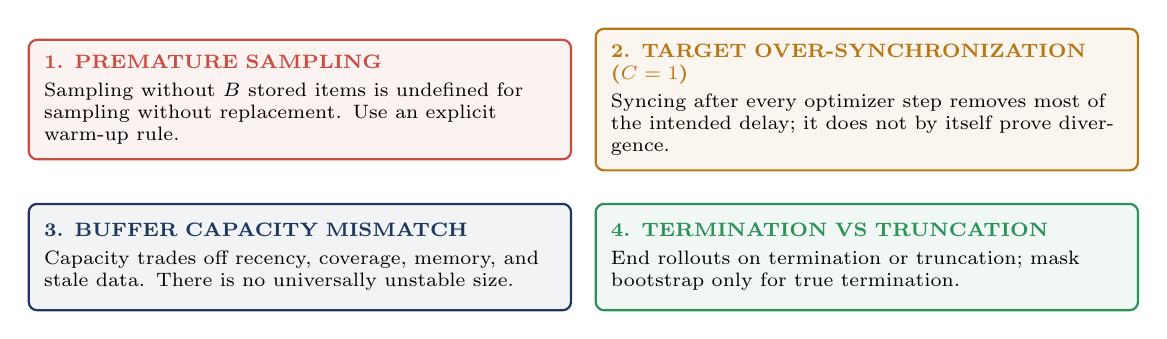
\begin{tikzpicture}[
      card/.style={rounded corners=3pt, text width=6.5cm, minimum height=1.35cm, align=left, inner sep=5.5pt, font=\scriptsize, line width=0.8pt}
    ]
      \node[card, draw=islred, fill=islred!7] at (3.5, 3.3) {
        {\bfseries\color{islred} 1. PREMATURE SAMPLING}\\[2pt]
        Sampling without $B$ stored items is undefined for sampling without replacement. Use an explicit warm-up rule.
      };

      \node[card, draw=islgold, fill=islgold!7] at (10.7, 3.3) {
        {\bfseries\color{islgold} 2. TARGET OVER-SYNCHRONIZATION ($C=1$)}\\[2pt]
        Syncing after every optimizer step removes most of the intended delay; it does not by itself prove divergence.
      };

      \node[card, draw=islnavy, fill=islnavy!6] at (3.5, 1.3) {
        {\bfseries\color{islnavy} 3. BUFFER CAPACITY MISMATCH}\\[2pt]
        Capacity trades off recency, coverage, memory, and stale data. There is no universally unstable size.
      };

      \node[card, draw=islgreen, fill=islgreen!7] at (10.7, 1.3) {
        {\bfseries\color{islgreen} 4. TERMINATION VS TRUNCATION}\\[2pt]
        End rollouts on termination or truncation; mask bootstrap only for true termination.
      };
    \end{tikzpicture}
  \end{center}
\end{frame}

% ==========================================
% SLIDE 9: Robotics Horizon Bridge
% ==========================================
\begin{frame}{Robotics Bridge: Off-Policy Sample Efficiency}
  \sectionlabel{Why replay buffers are the foundation of physical robot learning}

  \begin{columns}[T,onlytextwidth]
    \column{0.48\textwidth}
      {\small\bfseries\color{islnavy} The Physical Reality}\par\vspace{0.08cm}
      {\footnotesize
      $\bullet$ Physical execution is slower and costlier than model updates.\\[2pt]
      $\bullet$ Stored trials can support multiple optimizer steps.\\[2pt]
      $\bullet$ Report the update-to-data ratio and hardware interaction budget.}

    \column{0.48\textwidth}
      {\small\bfseries\color{islteal} Real-to-Sim \& Prioritized Buffers}\par\vspace{0.08cm}
      {\footnotesize
      $\bullet$ \textbf{Hybrid Buffers:} Mix real and simulated data deliberately, with proportions reported.\\[2pt]
      $\bullet$ \textbf{PER:} TD-error priorities are not identical to rarity, safety, or task importance.}
  \end{columns}
\end{frame}

% ==========================================
% SLIDE 10: Quiz Part 1 - Concepts Check
% ==========================================
\begin{frame}{Week 04 Quiz: Core Concepts \& Mechanisms}
  \sectionlabel{Self-check: verify fundamental understanding of replay buffers \& target networks}

  \begin{center}
    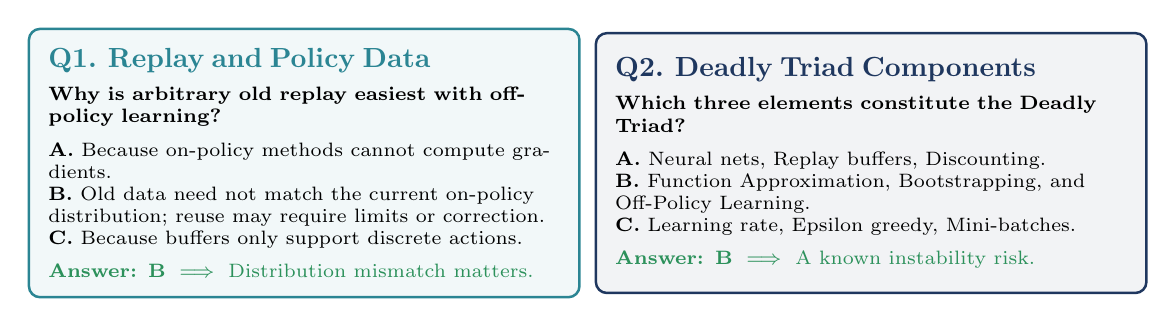
\begin{tikzpicture}[
      qcard/.style={rounded corners=4pt, text width=6.5cm, minimum height=3.3cm, align=left, inner sep=7pt, font=\scriptsize, line width=0.9pt}
    ]
      % Question 1
      \node[qcard, draw=islteal, fill=islteal!6] at (3.5, 1.7) {
        {\bfseries\color{islteal}\normalsize Q1. Replay and Policy Data}\\[4pt]
        \textbf{Why is arbitrary old replay easiest with off-policy learning?}\\[4pt]
        \textbf{A.} Because on-policy methods cannot compute gradients.\\
        \textbf{B.} Old data need not match the current on-policy distribution; reuse may require limits or correction.\\
        \textbf{C.} Because buffers only support discrete actions.
        \vskip4pt
        {\color{islgreen}\textbf{Answer: B} $\implies$ Distribution mismatch matters.}
      };

      % Question 2
      \node[qcard, draw=islnavy, fill=islnavy!6] at (10.7, 1.7) {
        {\bfseries\color{islnavy}\normalsize Q2. Deadly Triad Components}\\[4pt]
        \textbf{Which three elements constitute the Deadly Triad?}\\[4pt]
        \textbf{A.} Neural nets, Replay buffers, Discounting.\\
        \textbf{B.} Function Approximation, Bootstrapping, and Off-Policy Learning.\\
        \textbf{C.} Learning rate, Epsilon greedy, Mini-batches.
        \vskip4pt
        {\color{islgreen}\textbf{Answer: B} $\implies$ A known instability risk.}
      };
    \end{tikzpicture}
  \end{center}
\end{frame}

% ==========================================
% SLIDE 11: Quiz Part 2 - Buffer & Polyak Arithmetic
% ==========================================
\begin{frame}{Week 04 Quiz: Buffer \& Polyak Arithmetic}
  \sectionlabel{Verify hand-computations for replay indices and target update formulas}

  \begin{center}
    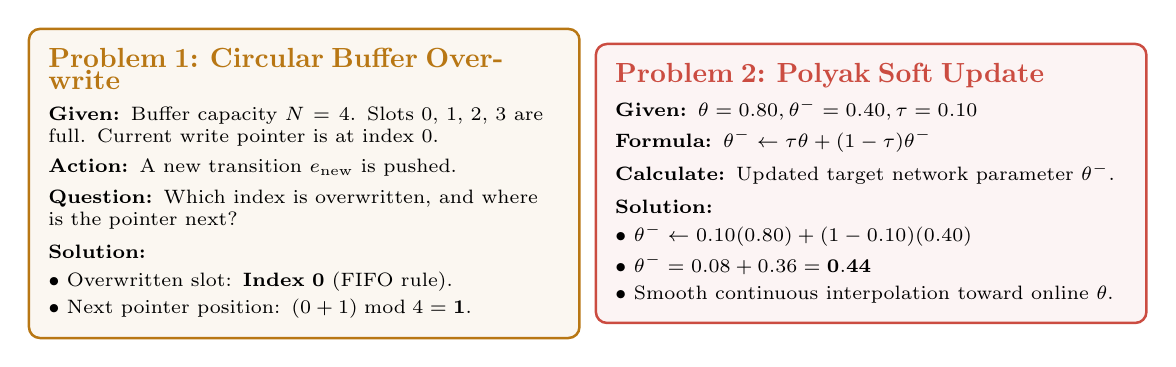
\begin{tikzpicture}[
      qcard/.style={rounded corners=4pt, text width=6.5cm, minimum height=3.3cm, align=left, inner sep=7pt, font=\scriptsize, line width=0.9pt}
    ]
      % Problem 1
      \node[qcard, draw=islgold, fill=islgold!6] at (3.5, 1.7) {
        {\bfseries\color{islgold}\normalsize Problem 1: Circular Buffer Overwrite}\\[3pt]
        \textbf{Given:} Buffer capacity $N=4$. Slots 0, 1, 2, 3 are full. Current write pointer is at index 0.\\[3pt]
        \textbf{Action:} A new transition $e_{\text{new}}$ is pushed.\\[3pt]
        \textbf{Question:} Which index is overwritten, and where is the pointer next?\\[4pt]
        \textbf{Solution:}\\[2pt]
        $\bullet$ Overwritten slot: \textbf{Index 0} (FIFO rule).\\[2pt]
        $\bullet$ Next pointer position: $(0 + 1) \bmod 4 = \mathbf{1}$.
      };

      % Problem 2
      \node[qcard, draw=islred, fill=islred!6] at (10.7, 1.7) {
        {\bfseries\color{islred}\normalsize Problem 2: Polyak Soft Update}\\[3pt]
        \textbf{Given:} $\theta = 0.80, \theta^- = 0.40, \tau = 0.10$\\[3pt]
        \textbf{Formula:} $\theta^- \leftarrow \tau \theta + (1 - \tau)\theta^-$\\[3pt]
        \textbf{Calculate:} Updated target network parameter $\theta^-$.\\[4pt]
        \textbf{Solution:}\\[2pt]
        $\bullet$ $\theta^- \leftarrow 0.10(0.80) + (1 - 0.10)(0.40)$\\[2pt]
        $\bullet$ $\theta^- = 0.08 + 0.36 = \mathbf{0.44}$\\[2pt]
        $\bullet$ Smooth continuous interpolation toward online $\theta$.
      };
    \end{tikzpicture}
  \end{center}
\end{frame}

% ==========================================
% SLIDE 12: Quiz Part 3 - Diagnostics & Traps
% ==========================================
\begin{frame}{Week 04 Quiz: Diagnostics \& Practical Traps}
  \sectionlabel{Key engineering questions every RL practitioner must master}

  \begin{center}
    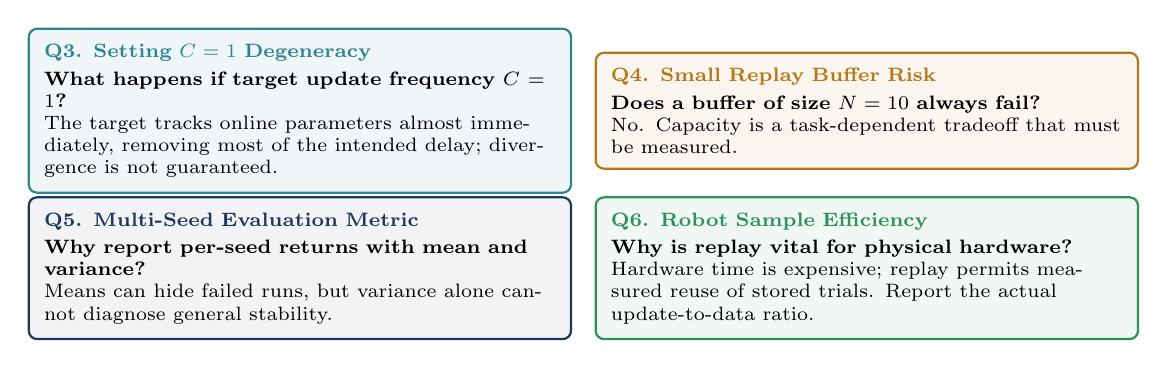
\begin{tikzpicture}[
      card/.style={rounded corners=3pt, text width=6.5cm, minimum height=1.35cm, align=left, inner sep=5.5pt, font=\scriptsize, line width=0.8pt}
    ]
      \node[card, draw=islteal, fill=islteal!7] at (3.5, 3.3) {
        {\bfseries\color{islteal} Q3. Setting $C=1$ Degeneracy}\\[2pt]
        \textbf{What happens if target update frequency $C=1$?}\\
        The target tracks online parameters almost immediately, removing most of the intended delay; divergence is not guaranteed.
      };

      \node[card, draw=islgold, fill=islgold!7] at (10.7, 3.3) {
        {\bfseries\color{islgold} Q4. Small Replay Buffer Risk}\\[2pt]
        \textbf{Does a buffer of size $N=10$ always fail?}\\
        No. Capacity is a task-dependent tradeoff that must be measured.
      };

      \node[card, draw=islnavy, fill=islnavy!6] at (3.5, 1.3) {
        {\bfseries\color{islnavy} Q5. Multi-Seed Evaluation Metric}\\[2pt]
        \textbf{Why report per-seed returns with mean and variance?}\\
        Means can hide failed runs, but variance alone cannot diagnose general stability.
      };

      \node[card, draw=islgreen, fill=islgreen!7] at (10.7, 1.3) {
        {\bfseries\color{islgreen} Q6. Robot Sample Efficiency}\\[2pt]
        \textbf{Why is replay vital for physical hardware?}\\
        Hardware time is expensive; replay permits measured reuse of stored trials. Report the actual update-to-data ratio.
      };
    \end{tikzpicture}
  \end{center}
\end{frame}

\end{document}
